\documentclass[a4paper]{article}

\usepackage[utf8]{inputenc}
\usepackage[T1]{fontenc}
\usepackage{textcomp}
\usepackage[dutch]{babel}
\usepackage{amsmath, amssymb}
\usepackage{ dsfont }
\usepackage{code}
\usepackage{pythonhighlight}
\usepackage{float}
% figure support
\usepackage{import}
\usepackage{xifthen}
\pdfminorversion=7
\usepackage{pdfpages}
\usepackage{transparent}
\usepackage{graphicx}
\pdfsuppresswarningpagegroup=1
\graphicspath{{./img/}}
\begin{document}
\section{Intro - lightboard}
Everything follows right hand rule
\begin{figure}[htpb]
	\centering
	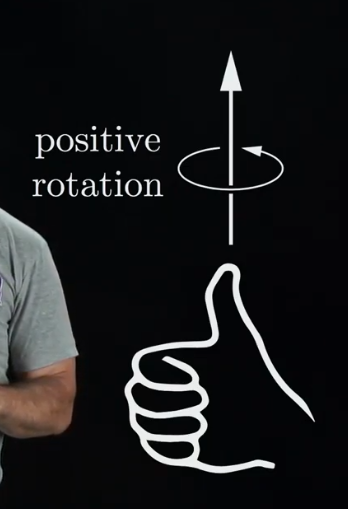
\includegraphics[width=0.5\textwidth]{postiveRotaion.png}
	\caption{}
	\label{fig:}
\end{figure}
\section{Foundation of mobile robotics ch-2}
\subsection{Degrees of freedom rigid body}
\begin{itemize}
	\item \textbf{Configuration} - A specific position of the position of all points of robot
	\item \textbf{C-space} - The space of all configuration
	\item \textbf{degrees of freedom} - dimension of c space
	\item Rigid body has 6 degrees of freedom

	\item dof - $\sum (freedom points) - no.of.constrains$ \\\
	      \begin{tabular}{|c|c|c|c|}
		      \hline
		      points  & dof & no.of.constrains & constrans       \\
		      \hline
		      point A & 2   & 0                & -               \\
		      point B & 2   & 1                & $d_{ab}$        \\
		      Point C & 2   & 2                & $d_{ac},{d_bc}$ \\
		      \hline
	      \end{tabular}
	\item $dof = m(N-1) - \sum_{i=1}^J c_i$
	\item also $c_i + f_i = m$
\end{itemize}
\subsubsection{Grublers formula}
\begin{itemize}
	\item N = no of links
	\item J = no of joints
	\item m = dof of rigid body (3 for planar 6 for spatial)
	\item $f_i$ = No of freedom of joint
	\item $c_i$ = No of constrains by joint
	\item \begin{align*}
		      Dof & = m(N-1) - \sum_{i=1}^j c_i                                          \\
		          & = m(N-1) \sum_{i=1}^j m-f_i     & \because m = f_i + c_i             \\
		          & = m(N-1) - J.m \sum_{i=1}^j f_i & \because \sum_{i=0}^j \bf{c} = J.c \\
		          & = m(N-1-J) + \sum_{i=1}^j f_i
	      \end{align*}
	\item Grubler formula is valid only for joints with independant constrain
	\item Closed chain mechanism - both base and end point is connected to ground
	      \begin{figure}[H]
		      \centering
		      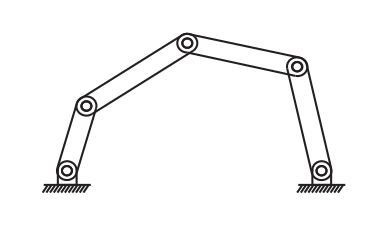
\includegraphics[width=0.8\textwidth]{closedchain.png}
		      \caption{}
		      \label{fig:}
	      \end{figure}
	\item Open chain mechanism only base is attached to ground
	      \begin{figure}[H]
		      \centering
		      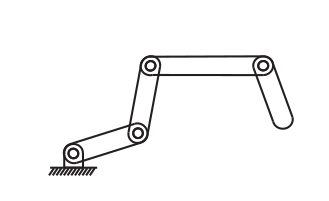
\includegraphics[width=0.8\textwidth]{openchain.png}
		      \caption{}
		      \label{fig:}
	      \end{figure}
\end{itemize}
\subsection{Configuration space topology}
\begin{itemize}
	\item sphere and plance has same dimension (x,y and latitude,longitude) but diffrent hape
	\item shape of the c-space is \textbf{topology}
	\item \textbf{Topologically equivalent}  - if two spaces can be deformed into each other without any removal or addition
	\item $\mathds{E}^1$ - euclidean line
	\item c space can be expressed as \textbf{cartesian product} of two are more space of lower dimension
	\item c- space of some common robots ($X^n$ where n is the dimension)
	      \begin{itemize}
		      \item Rigid body in plane = $\mathds{R}^2 \times \mathds{S}^1 $
		      \item PR robot arm = $\mathds{R}^1 \times \mathds{S}^1$
		      \item planar rigid body with PR arm = \begin{align*}
			            \text{for arm}         & = \mathds{S}^1 \times \mathds{S}^1 = T^2               & \ldots \text{T = torus} \\
			            \text{for mobile base} & =  \mathds{R}^2 \times \mathds{S}^1                                              \\
			            \therefore c-space     & = \mathds{R}^2 \times \mathds{S}^1 \times \mathds{T}^2                           \\
			                                   & = \mathds{R}^2 \times T^3
		            \end{align*}
	      \end{itemize}
\end{itemize}
\subsection{Configure space Representation}
To perform computations we need numerical represenstation
\subsubsection{Explicit represenstation}
\begin{itemize}
	\item choice of n co-ordinates for to represent an n-dimensional space
	\item for sphere,longitude and latitude
	\item causes singularaties (at northpole,sudden shift in values)
	\item to avoid this use co-ordinate  chart(split parts like atlas)
\end{itemize}
\subsubsection{Implicit represenstation}
\begin{itemize}
	\item represensting n n-dimensional space as if it is embedded in euclidean space
	\item disadvantage as has more variable to consider
	\item easy to define closed loops
\end{itemize}
\subsection{Configuration and velocity constrain}
For a 4 bar linkage,the closed loop can be expressed by the following equations
\begin{align*}
	L_1\cos\theta_1+L_2\cos(\theta_1 + \theta_2) + \ldots +L_4\cos(\theta_1+\ldots+\theta_4) & = 0                                                      \\
	L_1\sin\theta_1+L_2\sin(\theta_1 + \theta_2) + \ldots +L_4\sin(\theta_1+\ldots+\theta_4) & = 0 & \because \text{sum of all vectors in loop is zero} \\
	\theta_1 + \theta_2 + \theta_3 + \theta_4 + 2 \pi                                        & = 0 & \because \text{sum of all angles is $2\pi$}
\end{align*}
These equations are called \textbf{loop closure equations}.For general robots c-space can be implicitly represented by column vector $\theta = \begin{bmatrix} \theta_1 & \ldots & \theta_n\end{bmatrix}^T \in \mathds{R}^n$
\begin{equation}
	g(\theta) = \begin{bmatrix}
		g_1(\theta_1,\ldots,theta_n) \\
		\vdots                       \\
		\g_k(\theta_1,\ldots,\theta_k)
	\end{bmatrix} = 0
\end{equation}
By diffrentiating the above equation \footnote{find how this happened?}
            \begin{figure}[H]
                                    \centering
                                    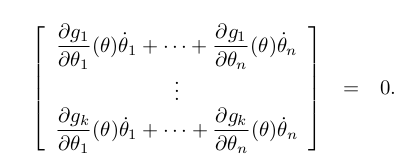
\includegraphics[width=0.8\textwidth]{equationofclosedloop.png}
                                    \caption{}
                                    \label{fig:}
                                \end{figure}
        this can be expressed as matrix multiplying a column vector
        \begin{figure}[H]
                                        \centering
                                        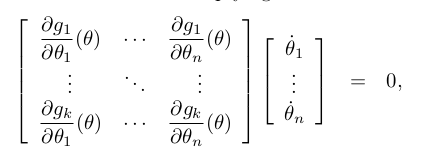
\includegraphics[width=0.8\textwidth]{equationofclosedloopasmatrix.png}
                                        \caption{}
                                        \label{fig:}
                                    \end{figure}
\end{document}
